\begin{enumerate}[label=\thesubsection.\arabic*.,ref=\thesubsection.\theenumi]
\numberwithin{equation}{enumi}

\item In the block diagram Fig.\ref{fig:ee18btech11029}  
\begin{align}
G\brak{s} = \frac{K}{\brak{s+4}\brak{s+5}}
\label{ee18btech11034_Gs}
\end{align}
\begin{figure}[!ht]
    \begin{center}
		\resizebox{\columnwidth}{!}{\tikzset{
        block/.style = {draw, rectangle,
            minimum height=1cm,
            minimum width=2cm},
        input/.style = {coordinate,node distance=1cm},
        output/.style = {coordinate,node distance=4cm},
        arrow/.style={draw, -latex,node distance=2cm},
        pinstyle/.style = {pin edge={latex-, black,node distance=2cm}},
        sum/.style = {draw, circle, node distance=1cm},
}

\begin{tikzpicture}[node distance=2.5cm,auto,>=latex']
  \node [input, name=input] {};
  \node [sum, right = 1cm of input] (sum) {};
  \node [block, right =0.5 cm of sum] (block1) {$G(s)$};
  \node [sum,right  = 0.7 cm of block1] (sum1){};
  \node [input ,right =0.25cm of block1] (p1) {};
  \node [input ,below = 1 cm of p1] (p2){};
  \node [input ,left = 2.7cm of p2] (p3){};
  \node [input ,above =0.8cm of p3] (p4) {};
  \node [block,right  = 0.5 cm of sum1] (block2) {$G(s)$};
  \node [input ,right =0.25cm of block2] (q1) {};
  \node [input ,below = 1 cm of q1] (q2){};
  \node [input ,left = 2.8cm of q2] (q3){};
  \node [input ,above =0.7cm of q3] (q4) {};
   \node [input ,right =0.8cm of block2] (q5) {};
   \node [input ,below =1.5cm of q5] (q6){};
    \node [input ,left =7.24cm of q6] (q7){};
    \node [input ,above =0.9cm of q7] (q8) {};
    \node [input ,right =1cm of q5] (q9) {};
  
  
  
  
 
  
  
  \draw [->] (input) -- node {$R(s)\ +$} (sum);
  \draw [->] (sum) --  (block1);
 \draw [-]  (block1) -- (sum1);
 \draw [-]  (sum1) -- (block2);
 \draw [-]  (p1) -- (p2);
 \draw [-] (p2) -- (p3);
   \draw [->](p3) -| node[pos=0.90] {$-$} (p4);
  \draw [-] (block2) -- (q1);
  \draw[-] (q1) -- (q2);
  \draw[-] (q2) -- (q3);
  \draw [->](q3) -| node[pos=0.99] {$-$} (q4);
  \draw[-] (block2)--(q5);
   \draw[-] (q5) -- (q6);
    \draw[-] (q6) -- (q7);
  \draw [->](q7) -| node[pos=0.99] {$+$} (q8);
  \draw [->] (q5) -- node {$Y(s)$} (q9);

  %\draw [->] (block1) -- node {} (block2);
%  \draw [->] (block2) -- node [name =y] {$Y(s)$} (output);
 % \draw [->] (y) -- ++ (0,-2) -| node [pos=0.99] {$-$} (sum);

\end{tikzpicture}
}
	\end{center}
\caption{}
\label{fig:ee18btech11029}
\end{figure}
\item Find the range of K for stability by Nyquist criterion

\solution
\begin{figure}[!h]
    \begin{center}
		\resizebox{\columnwidth}{!}{\input{./figs/ee18btech11029/ee18btech11029_2.tex}}
	\end{center}
\caption{}
\label{fig:ee18btech11029_1}
\end{figure}


The open loop transfer function from Fig.\ref{fig:ee18btech11029_1}

\begin{align}
    T\brak{s} =\brak{\frac{\frac{K}{\brak{s+4}\brak{s+5}}}{1+\frac{K}{\brak{s+4}\brak{s+5}}}}^2 
\end{align}


\begin{align}
    T\brak{\j\omega} =\brak{\frac{\frac{K}{\brak{\j\omega+4}\brak{\j\omega+5}}}{1+\frac{K}{\brak{\j\omega+4}\brak{\j\omega+5}}}}^2 
\end{align}




\begin{itemize}
    \item Since it is connected in positive feedback the transfer function cuts at \brak{1,\j0} 
\end{itemize}

\begin{align}
    \implies  \text{Re} \cbrak{T\brak{\j\omega}} &= 1\\
      \implies  \text{Im} \cbrak{T\brak{\j \omega}} &= 0
     \label{eq:ee18btech11029_eq_Re}
\end{align}


\begin{align}
    \brak{\frac{\frac{K}{\brak{\j\omega+4}\brak{\j\omega+5}}}{1+\frac{K}{\brak{\j\omega+4}\brak{\j\omega+5}}}}^2 &= 1+\j0
\end{align}

\begin{align}
    \brak{\j\omega+4}\brak{\j\omega+5}+2K &=0
\end{align}

\begin{align}
    -\omega^2 + 9\j\omega +20+2K &=0 
\end{align}
\\
From  \eqref{eq:ee18btech11029_eq_Re}

\begin{align}
    20 + 2K &= 0\\
    \implies K=-10
\end{align}
The minimum value of stability for the system to be stable is
\begin{align}
    K_{min} > -10
\end{align}
The range of K for which the system is stable is 
\begin{align}
    -10 < K < \infty
\end{align}


\item From the table.\ref{table:ee18btech11029_table1}, 
Stability criterion for K is N+P=Z


\begin{table}[!h]
\centering
\input{./tables/ee18btech11029_table.tex}
\caption{}
\label{table:ee18btech11029_table1}
\end{table}


\item Verify the Nyquist plots by
\begin{lstlisting}
codes/ee18btech11029_1.py
\end{lstlisting}


\begin{figure}[h!]
\centering
  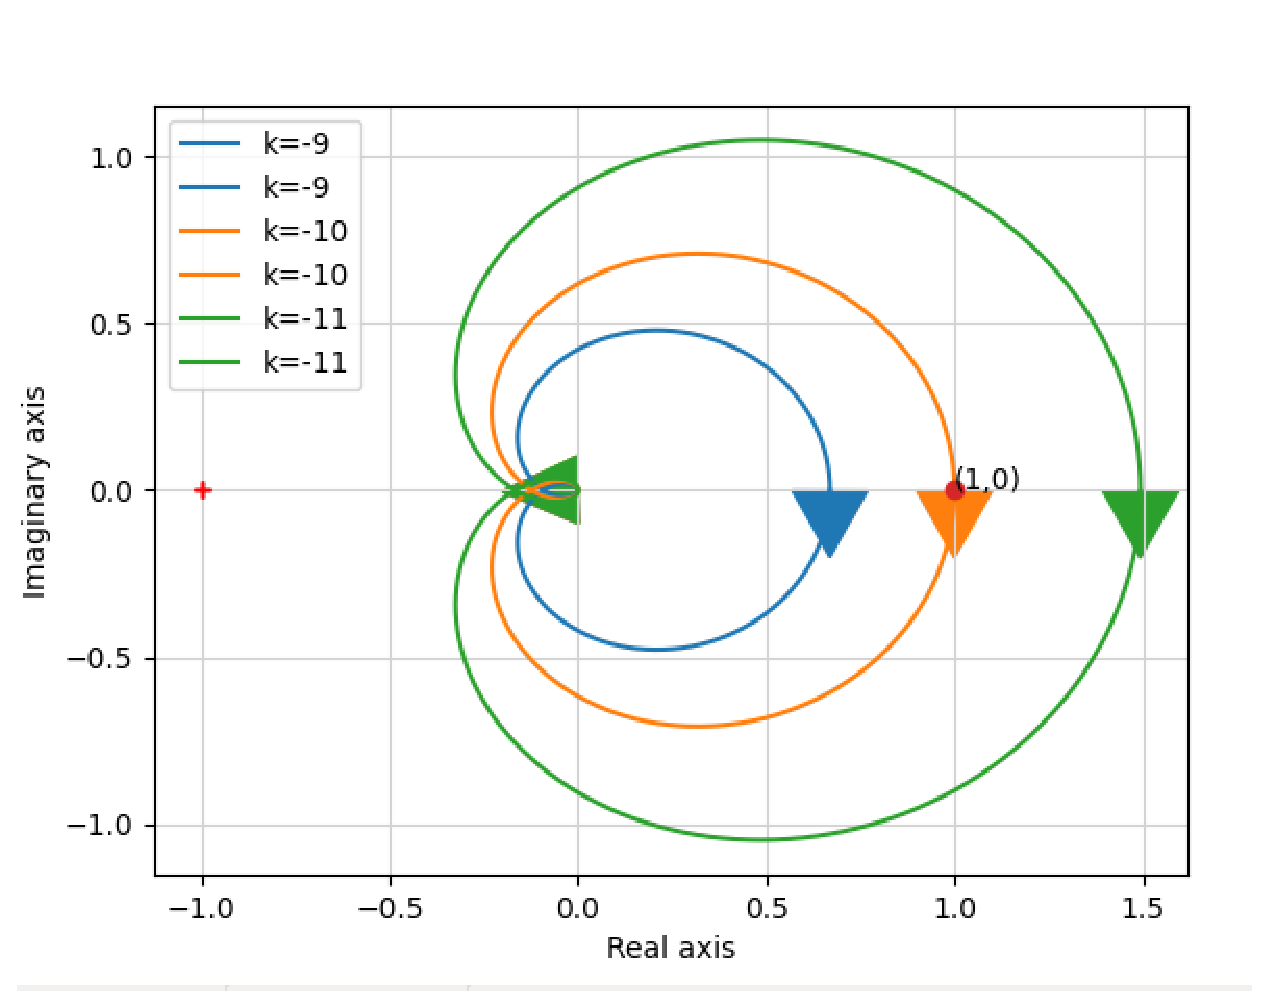
\includegraphics[width=\columnwidth]{./figs/ee18btech11029/Nyquist.eps}
  \caption{Nyquist Plot}
  \label{fig:ee18btech11029_2}
\end{figure}





\item Verify the result using Routh-Hurwitz criterion

\solution The characteristic equation is 
\begin{align}
    1-T\brak{s} &=0\\
    1-\brak{\frac{\frac{K}{\brak{s+4}\brak{s+5}}}{1+\frac{K}{\brak{s+4}\brak{s+5}}}}^2 &=0\\
    1+2\brak{\frac{K}{\brak{s+4}\brak{s+5}}}&=0\\
    s^2+9s+20+2K &= 0
\end{align}

\begin{align}
\mydet{s^2\\s^1\\s^0}
\mydet{1 & 20+2K \\ 9 & 0 \\ 20+2K & 0}
\end{align}
For a system to be stable it should not have any sign changes
\begin{align}
    20+2K >0
\end{align}
This is valid for all positive values of K but the minimum value of K is
\begin{align}
    K>-10
\end{align}
So the range of K for stability is 
\begin{align}
    -10<K<\infty
\end{align}

\item Verify the result by
\begin{lstlisting}
codes/ee18btech11029_2.py
\end{lstlisting}







\end{enumerate}
